\documentclass[twoside]{book}

% Packages required by doxygen
\usepackage{calc}
\usepackage{doxygen}
\usepackage{graphicx}
\usepackage[utf8]{inputenc}
\usepackage{makeidx}
\usepackage{multicol}
\usepackage{multirow}
\usepackage{textcomp}
\usepackage[table]{xcolor}

% Font selection
\usepackage[T1]{fontenc}
\usepackage{mathptmx}
\usepackage[scaled=.90]{helvet}
\usepackage{courier}
\usepackage{amssymb}
\usepackage{sectsty}
\renewcommand{\familydefault}{\sfdefault}
\allsectionsfont{%
  \fontseries{bc}\selectfont%
  \color{darkgray}%
}
\renewcommand{\DoxyLabelFont}{%
  \fontseries{bc}\selectfont%
  \color{darkgray}%
}

% Page & text layout
\usepackage{geometry}
\geometry{%
  a4paper,%
  top=2.5cm,%
  bottom=2.5cm,%
  left=2.5cm,%
  right=2.5cm%
}
\tolerance=750
\hfuzz=15pt
\hbadness=750
\setlength{\emergencystretch}{15pt}
\setlength{\parindent}{0cm}
\setlength{\parskip}{0.2cm}
\makeatletter
\renewcommand{\paragraph}{%
  \@startsection{paragraph}{4}{0ex}{-1.0ex}{1.0ex}{%
    \normalfont\normalsize\bfseries\SS@parafont%
  }%
}
\renewcommand{\subparagraph}{%
  \@startsection{subparagraph}{5}{0ex}{-1.0ex}{1.0ex}{%
    \normalfont\normalsize\bfseries\SS@subparafont%
  }%
}
\makeatother

% Headers & footers
\usepackage{fancyhdr}
\pagestyle{fancyplain}
\fancyhead[LE]{\fancyplain{}{\bfseries\thepage}}
\fancyhead[CE]{\fancyplain{}{}}
\fancyhead[RE]{\fancyplain{}{\bfseries\leftmark}}
\fancyhead[LO]{\fancyplain{}{\bfseries\rightmark}}
\fancyhead[CO]{\fancyplain{}{}}
\fancyhead[RO]{\fancyplain{}{\bfseries\thepage}}
\fancyfoot[LE]{\fancyplain{}{}}
\fancyfoot[CE]{\fancyplain{}{}}
\fancyfoot[RE]{\fancyplain{}{\bfseries\scriptsize Generated on Tue Nov 17 2015 20\-:15\-:34 for M\-P\-A\-G\-S-\/\-Cipher by Doxygen }}
\fancyfoot[LO]{\fancyplain{}{\bfseries\scriptsize Generated on Tue Nov 17 2015 20\-:15\-:34 for M\-P\-A\-G\-S-\/\-Cipher by Doxygen }}
\fancyfoot[CO]{\fancyplain{}{}}
\fancyfoot[RO]{\fancyplain{}{}}
\renewcommand{\footrulewidth}{0.4pt}
\renewcommand{\chaptermark}[1]{%
  \markboth{#1}{}%
}
\renewcommand{\sectionmark}[1]{%
  \markright{\thesection\ #1}%
}

% Indices & bibliography
\usepackage{natbib}
\usepackage[titles]{tocloft}
\setcounter{tocdepth}{3}
\setcounter{secnumdepth}{5}
\makeindex

% Hyperlinks (required, but should be loaded last)
\usepackage{ifpdf}
\ifpdf
  \usepackage[pdftex,pagebackref=true]{hyperref}
\else
  \usepackage[ps2pdf,pagebackref=true]{hyperref}
\fi
\hypersetup{%
  colorlinks=true,%
  linkcolor=blue,%
  citecolor=blue,%
  unicode%
}

% Custom commands
\newcommand{\clearemptydoublepage}{%
  \newpage{\pagestyle{empty}\cleardoublepage}%
}


%===== C O N T E N T S =====

\begin{document}

% Titlepage & ToC
\hypersetup{pageanchor=false}
\pagenumbering{roman}
\begin{titlepage}
\vspace*{7cm}
\begin{center}%
{\Large M\-P\-A\-G\-S-\/\-Cipher \\[1ex]\large v1.\-0.\-1 }\\
\vspace*{1cm}
{\large Generated by Doxygen 1.8.6}\\
\vspace*{0.5cm}
{\small Tue Nov 17 2015 20:15:34}\\
\end{center}
\end{titlepage}
\clearemptydoublepage
\tableofcontents
\clearemptydoublepage
\pagenumbering{arabic}
\hypersetup{pageanchor=true}

%--- Begin generated contents ---
\chapter{Hierarchical Index}
\section{Class Hierarchy}
This inheritance list is sorted roughly, but not completely, alphabetically\-:\begin{DoxyCompactList}
\item \contentsline{section}{Caesar\-Cipher}{\pageref{class_caesar_cipher}}{}
\item \contentsline{section}{Command\-Line\-Info}{\pageref{struct_command_line_info}}{}
\item exception\begin{DoxyCompactList}
\item \contentsline{section}{Help\-Exception}{\pageref{class_help_exception}}{}
\item \contentsline{section}{help\-Exception}{\pageref{classhelp_exception}}{}
\item \contentsline{section}{version\-Exception}{\pageref{classversion_exception}}{}
\end{DoxyCompactList}
\item \contentsline{section}{my\-Stop}{\pageref{structmy_stop}}{}
\item \contentsline{section}{Playfair\-Cipher}{\pageref{class_playfair_cipher}}{}
\item \contentsline{section}{Version\-Exception}{\pageref{struct_version_exception}}{}
\item \contentsline{section}{Vigenere\-Cipher}{\pageref{class_vigenere_cipher}}{}
\end{DoxyCompactList}

\chapter{Class Index}
\section{Class List}
Here are the classes, structs, unions and interfaces with brief descriptions\-:\begin{DoxyCompactList}
\item\contentsline{section}{\hyperlink{class_caesar_cipher}{Caesar\-Cipher} }{\pageref{class_caesar_cipher}}{}
\item\contentsline{section}{\hyperlink{struct_command_line_info}{Command\-Line\-Info} \\*Structure to hold the information passed into the command line by the user }{\pageref{struct_command_line_info}}{}
\item\contentsline{section}{\hyperlink{classhelp_exception}{help\-Exception} }{\pageref{classhelp_exception}}{}
\item\contentsline{section}{\hyperlink{class_help_exception}{Help\-Exception} }{\pageref{class_help_exception}}{}
\item\contentsline{section}{\hyperlink{structmy_stop}{my\-Stop} }{\pageref{structmy_stop}}{}
\item\contentsline{section}{\hyperlink{class_playfair_cipher}{Playfair\-Cipher} }{\pageref{class_playfair_cipher}}{}
\item\contentsline{section}{\hyperlink{classversion_exception}{version\-Exception} }{\pageref{classversion_exception}}{}
\item\contentsline{section}{\hyperlink{struct_version_exception}{Version\-Exception} }{\pageref{struct_version_exception}}{}
\item\contentsline{section}{\hyperlink{class_vigenere_cipher}{Vigenere\-Cipher} }{\pageref{class_vigenere_cipher}}{}
\end{DoxyCompactList}

\chapter{Class Documentation}
\hypertarget{class_caesar_cipher}{\section{Caesar\-Cipher Class Reference}
\label{class_caesar_cipher}\index{Caesar\-Cipher@{Caesar\-Cipher}}
}


{\ttfamily \#include $<$Caesar\-Cipher.\-hpp$>$}

\subsection*{Public Member Functions}
\begin{DoxyCompactItemize}
\item 
\hyperlink{class_caesar_cipher_aac0c030f098c6aef23d3a6b596aaf4aa}{Caesar\-Cipher} (std\-::string constructorkey, Cipher\-Mode mode)
\item 
int \hyperlink{class_caesar_cipher_a53b507960879e111df84de87da4bd1fd}{wrap\-It} (int index)
\item 
char \hyperlink{class_caesar_cipher_a60e50b9f5b32756b44d986fe1901eacb}{shift} (char input)
\item 
std\-::string \hyperlink{class_caesar_cipher_a7990118b655a6001aaf34824de9241e7}{encrypt} (std\-::string msg)
\item 
\hypertarget{class_caesar_cipher_a85dc304c1762e6e86ac5b1d0193d1ac7}{void {\bfseries make\-It\-Look\-Nice} (std\-::string \&msg)}\label{class_caesar_cipher_a85dc304c1762e6e86ac5b1d0193d1ac7}

\end{DoxyCompactItemize}
\subsection*{Public Attributes}
\begin{DoxyCompactItemize}
\item 
\hypertarget{class_caesar_cipher_ac515c66e4c5b0e01205d32a5e33bf77e}{const std\-::vector$<$ char $>$ {\bfseries alphabet\-\_\-}}\label{class_caesar_cipher_ac515c66e4c5b0e01205d32a5e33bf77e}

\item 
\hypertarget{class_caesar_cipher_afd4c56635dd54fe2b4b503362ce99abc}{const int {\bfseries key\-\_\-} = 0}\label{class_caesar_cipher_afd4c56635dd54fe2b4b503362ce99abc}

\item 
\hypertarget{class_caesar_cipher_a6258687dec40287b19bc1ffe1a305975}{const Cipher\-Mode {\bfseries mode\-\_\-} = Cipher\-Mode\-::\-Encrypt}\label{class_caesar_cipher_a6258687dec40287b19bc1ffe1a305975}

\end{DoxyCompactItemize}


\subsection{Detailed Description}
\hyperlink{class_caesar_cipher}{Caesar\-Cipher} contains the alphabet, the key of the cipher and a flag for decryption 

\subsection{Constructor \& Destructor Documentation}
\hypertarget{class_caesar_cipher_aac0c030f098c6aef23d3a6b596aaf4aa}{\index{Caesar\-Cipher@{Caesar\-Cipher}!Caesar\-Cipher@{Caesar\-Cipher}}
\index{Caesar\-Cipher@{Caesar\-Cipher}!CaesarCipher@{Caesar\-Cipher}}
\subsubsection[{Caesar\-Cipher}]{\setlength{\rightskip}{0pt plus 5cm}Caesar\-Cipher\-::\-Caesar\-Cipher (
\begin{DoxyParamCaption}
\item[{std\-::string}]{constructorkey, }
\item[{Cipher\-Mode}]{mode}
\end{DoxyParamCaption}
)}}\label{class_caesar_cipher_aac0c030f098c6aef23d3a6b596aaf4aa}
Create a new \hyperlink{class_caesar_cipher}{Caesar\-Cipher}


\begin{DoxyParams}{Parameters}
{\em key} & the key to the cipher. \\
\hline
{\em decrypt} & the flag, true is decrypt \\
\hline
\end{DoxyParams}

\begin{DoxyCode}
10   :alphabet\_\{\textcolor{charliteral}{'A'},\textcolor{charliteral}{'B'},\textcolor{charliteral}{'C'},\textcolor{charliteral}{'D'},\textcolor{charliteral}{'E'},\textcolor{charliteral}{'F'},\textcolor{charliteral}{'G'},\textcolor{charliteral}{'H'},\textcolor{charliteral}{'I'},\textcolor{charliteral}{'J'},\textcolor{charliteral}{'K'},\textcolor{charliteral}{'L'},\textcolor{charliteral}{'M'},\textcolor{charliteral}{'N'},\textcolor{charliteral}{'O'},\textcolor{charliteral}{'P'},\textcolor{charliteral}{'Q'},\textcolor{charliteral}{'R'},\textcolor{charliteral}{'S'},\textcolor{charliteral}{'T'},\textcolor{charliteral}{'U'},\textcolor{charliteral}{'V'},\textcolor{charliteral}{'W'},\textcolor{charliteral}{
      'X'},\textcolor{charliteral}{'Y'},\textcolor{charliteral}{'Z'}\}, key\_\{std::stoi(thekey)\},mode\_\{decrypt\_mode\}
11    \{
12    \}
\end{DoxyCode}


\subsection{Member Function Documentation}
\hypertarget{class_caesar_cipher_a7990118b655a6001aaf34824de9241e7}{\index{Caesar\-Cipher@{Caesar\-Cipher}!encrypt@{encrypt}}
\index{encrypt@{encrypt}!CaesarCipher@{Caesar\-Cipher}}
\subsubsection[{encrypt}]{\setlength{\rightskip}{0pt plus 5cm}std\-::string Caesar\-Cipher\-::encrypt (
\begin{DoxyParamCaption}
\item[{std\-::string}]{msg}
\end{DoxyParamCaption}
)}}\label{class_caesar_cipher_a7990118b655a6001aaf34824de9241e7}
\begin{DoxyReturn}{Returns}
the encrypted/decrypted string 
\end{DoxyReturn}

\begin{DoxyParams}{Parameters}
{\em msg} & the message to be used \\
\hline
\end{DoxyParams}

\begin{DoxyCode}
49                                             \{
50 
51     std::string output\{\};
52     
53     \textcolor{keywordflow}{for}(\textcolor{keywordtype}{size\_t} i=0; i < msg.length() ;i++)\{
54       output += \hyperlink{class_caesar_cipher_a60e50b9f5b32756b44d986fe1901eacb}{shift}(msg[i]);
55     \}
56     \textcolor{keywordflow}{return} output;
57    \}    
\end{DoxyCode}
\hypertarget{class_caesar_cipher_a60e50b9f5b32756b44d986fe1901eacb}{\index{Caesar\-Cipher@{Caesar\-Cipher}!shift@{shift}}
\index{shift@{shift}!CaesarCipher@{Caesar\-Cipher}}
\subsubsection[{shift}]{\setlength{\rightskip}{0pt plus 5cm}char Caesar\-Cipher\-::shift (
\begin{DoxyParamCaption}
\item[{char}]{input}
\end{DoxyParamCaption}
)}}\label{class_caesar_cipher_a60e50b9f5b32756b44d986fe1901eacb}
\begin{DoxyReturn}{Returns}
the shifted character 
\end{DoxyReturn}

\begin{DoxyParams}{Parameters}
{\em input} & the inputted character \\
\hline
\end{DoxyParams}

\begin{DoxyCode}
26                                   \{
27 
28     \textcolor{keywordtype}{int} index\{0\};
29     \textcolor{keywordtype}{int} shifter = key\_;
30  
31     \textcolor{comment}{//decryption shifts the other way}
32     \textcolor{keywordflow}{if}(mode\_ == CipherMode::Decrypt) \{
33       shifter = -key\_;\}
34 
35     \textcolor{comment}{//finds the index of the current char}
36     \textcolor{keywordflow}{for}(\textcolor{keywordtype}{size\_t} i =0; i < alphabet\_.size(); i++)\{
37       \textcolor{keywordflow}{if}( input == alphabet\_[i])\{
38     index = i;  
39       \}
40     \}
41     
42     \textcolor{comment}{//return the char from a shifted position}
43       \textcolor{keywordflow}{return} alphabet\_[ \hyperlink{class_caesar_cipher_a53b507960879e111df84de87da4bd1fd}{wrapIt}(index + shifter) ];
44   \}
\end{DoxyCode}
\hypertarget{class_caesar_cipher_a53b507960879e111df84de87da4bd1fd}{\index{Caesar\-Cipher@{Caesar\-Cipher}!wrap\-It@{wrap\-It}}
\index{wrap\-It@{wrap\-It}!CaesarCipher@{Caesar\-Cipher}}
\subsubsection[{wrap\-It}]{\setlength{\rightskip}{0pt plus 5cm}int Caesar\-Cipher\-::wrap\-It (
\begin{DoxyParamCaption}
\item[{int}]{index}
\end{DoxyParamCaption}
)}}\label{class_caesar_cipher_a53b507960879e111df84de87da4bd1fd}
\begin{DoxyReturn}{Returns}
an index in range \mbox{[}0,25\mbox{]} 
\end{DoxyReturn}

\begin{DoxyParams}{Parameters}
{\em index} & the index to be wrapped \\
\hline
\end{DoxyParams}

\begin{DoxyCode}
17                                  \{
18 
19     \textcolor{keywordflow}{if}(index < 0)\{ index += 26;\}
20     \textcolor{keywordflow}{if}(index > 25)\{ index -= 26;\}
21 
22     \textcolor{keywordflow}{return} index;
23   \}
\end{DoxyCode}


The documentation for this class was generated from the following files\-:\begin{DoxyCompactItemize}
\item 
M\-P\-A\-G\-S\-Cipher/Caesar\-Cipher.\-hpp\item 
M\-P\-A\-G\-S\-Cipher/Caesar\-Cipher.\-cpp\end{DoxyCompactItemize}

\hypertarget{struct_command_line_info}{\section{Command\-Line\-Info Struct Reference}
\label{struct_command_line_info}\index{Command\-Line\-Info@{Command\-Line\-Info}}
}


Structure to hold the information passed into the command line by the user.  




{\ttfamily \#include $<$Process\-Command\-Line.\-hpp$>$}

\subsection*{Public Attributes}
\begin{DoxyCompactItemize}
\item 
\hypertarget{struct_command_line_info_ae5ba531705e89ae76a7346cbda8b4122}{bool {\bfseries help} = false}\label{struct_command_line_info_ae5ba531705e89ae76a7346cbda8b4122}

\item 
\hypertarget{struct_command_line_info_aa316bde21b3cc0e492a39d9cc8df918d}{bool {\bfseries version} = false}\label{struct_command_line_info_aa316bde21b3cc0e492a39d9cc8df918d}

\item 
\hypertarget{struct_command_line_info_ae50662480a9c2024db2475d9b74803a1}{Cipher\-Mode {\bfseries mode} = Cipher\-Mode\-::\-Encrypt}\label{struct_command_line_info_ae50662480a9c2024db2475d9b74803a1}

\item 
\hypertarget{struct_command_line_info_a33919bb28c7989eb80b6f5cff951ccd6}{std\-::string {\bfseries key}}\label{struct_command_line_info_a33919bb28c7989eb80b6f5cff951ccd6}

\item 
\hypertarget{struct_command_line_info_a26a4f338c4eef3d28708c589c4dcde57}{bool {\bfseries cipher\-\_\-err} = false}\label{struct_command_line_info_a26a4f338c4eef3d28708c589c4dcde57}

\item 
\hypertarget{struct_command_line_info_a3a669237126f9f2aaa1b360c80590164}{Cipher\-Type {\bfseries ciphertype}}\label{struct_command_line_info_a3a669237126f9f2aaa1b360c80590164}

\item 
\hypertarget{struct_command_line_info_aaa05222a62fbdcbf28bba04b0e973fb5}{std\-::string {\bfseries in\-\_\-file\-\_\-loc} = \char`\"{}\char`\"{}}\label{struct_command_line_info_aaa05222a62fbdcbf28bba04b0e973fb5}

\item 
\hypertarget{struct_command_line_info_a8c3888edf38e5b7e51bc5e3b3e13a07d}{std\-::string {\bfseries out\-\_\-file\-\_\-loc} = \char`\"{}\char`\"{}}\label{struct_command_line_info_a8c3888edf38e5b7e51bc5e3b3e13a07d}

\end{DoxyCompactItemize}


\subsection{Detailed Description}
Structure to hold the information passed into the command line by the user. 

The documentation for this struct was generated from the following file\-:\begin{DoxyCompactItemize}
\item 
M\-P\-A\-G\-S\-Cipher/Process\-Command\-Line.\-hpp\end{DoxyCompactItemize}

\hypertarget{classhelp_exception}{\section{help\-Exception Class Reference}
\label{classhelp_exception}\index{help\-Exception@{help\-Exception}}
}
Inheritance diagram for help\-Exception\-:\begin{figure}[H]
\begin{center}
\leavevmode
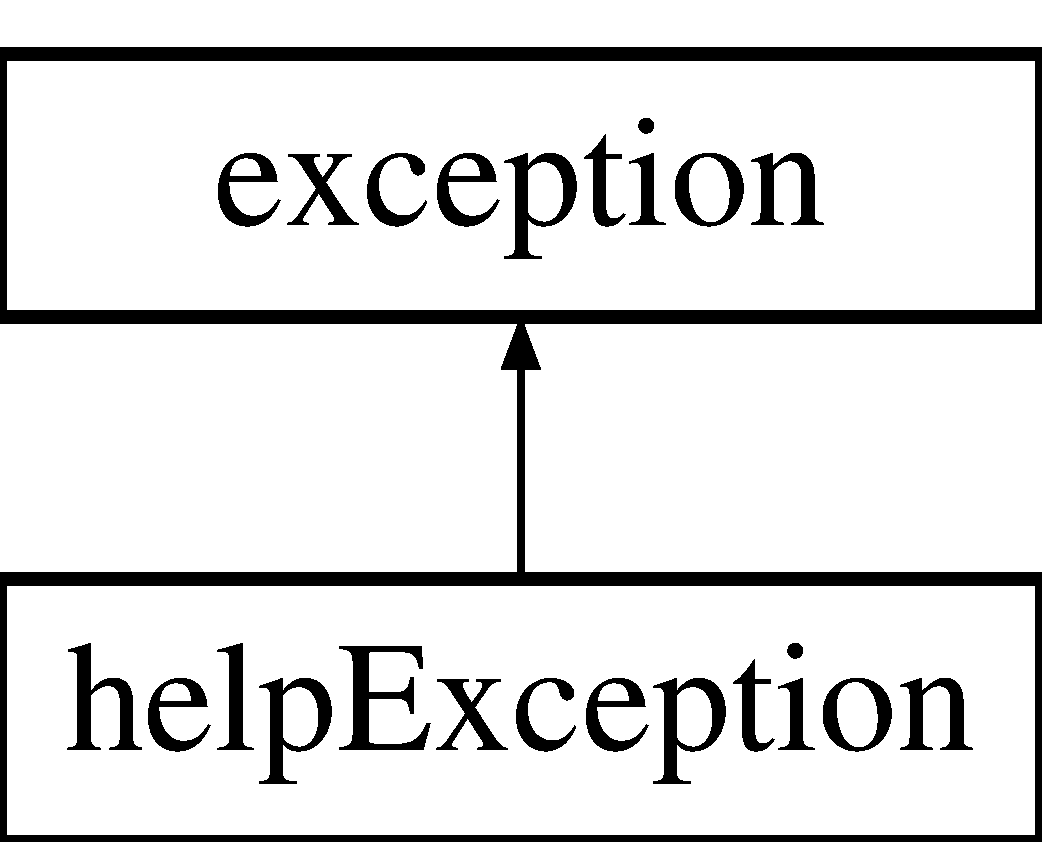
\includegraphics[height=2.000000cm]{classhelp_exception}
\end{center}
\end{figure}


The documentation for this class was generated from the following file\-:\begin{DoxyCompactItemize}
\item 
M\-P\-A\-G\-S\-Cipher/Command\-Line\-Helpers.\-cpp\end{DoxyCompactItemize}

\hypertarget{class_help_exception}{\section{Help\-Exception Class Reference}
\label{class_help_exception}\index{Help\-Exception@{Help\-Exception}}
}
Inheritance diagram for Help\-Exception\-:\begin{figure}[H]
\begin{center}
\leavevmode
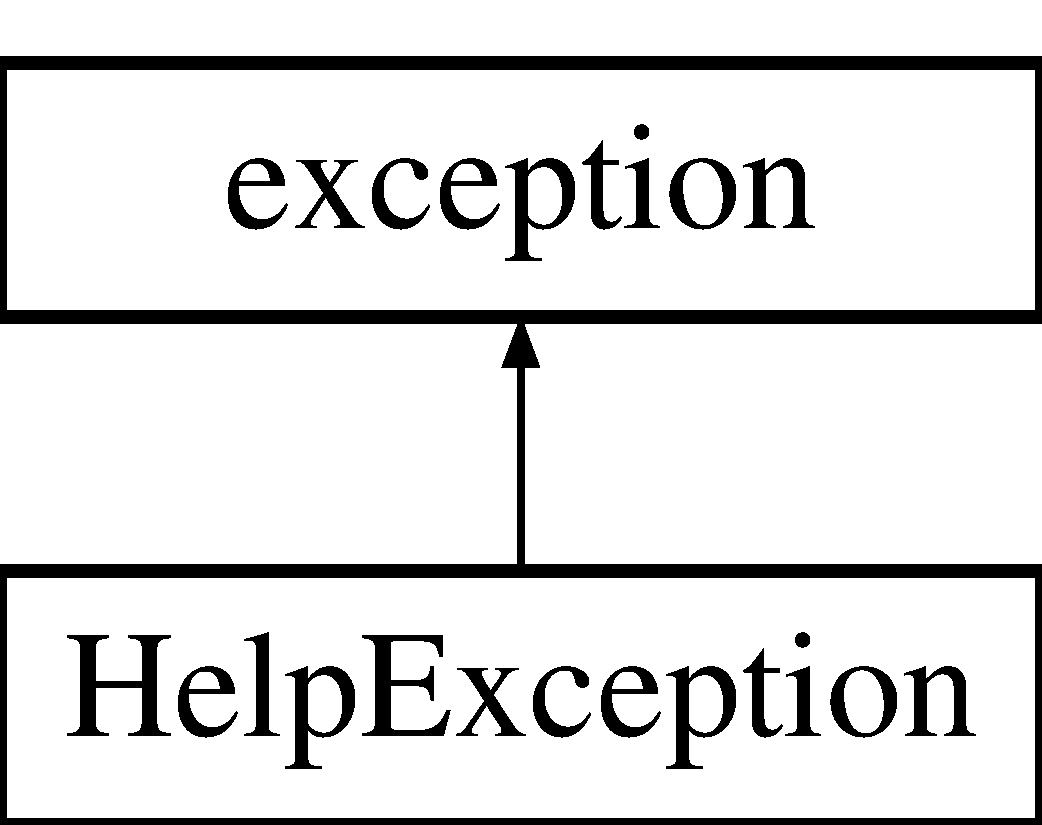
\includegraphics[height=2.000000cm]{class_help_exception}
\end{center}
\end{figure}
\subsection*{Public Member Functions}
\begin{DoxyCompactItemize}
\item 
\hypertarget{class_help_exception_af180aed08aeca8db0798de2ba23b3a18}{{\bfseries Help\-Exception} (const std\-::string m=\char`\"{}Help Called\char`\"{})}\label{class_help_exception_af180aed08aeca8db0798de2ba23b3a18}

\item 
\hypertarget{class_help_exception_aa486f90b62ddc54b614e54e69d7eec59}{const char $\ast$ {\bfseries what} ()}\label{class_help_exception_aa486f90b62ddc54b614e54e69d7eec59}

\end{DoxyCompactItemize}


The documentation for this class was generated from the following file\-:\begin{DoxyCompactItemize}
\item 
M\-P\-A\-G\-S\-Cipher/Custom\-Exceptions.\-cpp\end{DoxyCompactItemize}

\hypertarget{structmy_stop}{\section{my\-Stop Struct Reference}
\label{structmy_stop}\index{my\-Stop@{my\-Stop}}
}


The documentation for this struct was generated from the following file\-:\begin{DoxyCompactItemize}
\item 
M\-P\-A\-G\-S\-Cipher/Command\-Line\-Helpers.\-cpp\end{DoxyCompactItemize}

\hypertarget{class_playfair_cipher}{\section{Playfair\-Cipher Class Reference}
\label{class_playfair_cipher}\index{Playfair\-Cipher@{Playfair\-Cipher}}
}


{\ttfamily \#include $<$Playfair\-Cipher.\-hpp$>$}

\subsection*{Public Member Functions}
\begin{DoxyCompactItemize}
\item 
\hyperlink{class_playfair_cipher_a9547df4c76d947519d30355de7f00735}{Playfair\-Cipher} (std\-::string constructorkey, Cipher\-Mode mode)
\item 
void \hyperlink{class_playfair_cipher_a2c2d8f6b505f0d96cbff8124bcc00cc4}{set\-Key} (std\-::string key\-To\-Set)
\begin{DoxyCompactList}\small\item\em Creates the mapping from the keyword. \end{DoxyCompactList}\item 
int \hyperlink{class_playfair_cipher_aa16404acec63246dce3b30ea9dacb4cb}{play\-Wrap} (int index)
\begin{DoxyCompactList}\small\item\em A helper function to ensure coordinates are in the 5x5 square. \end{DoxyCompactList}\item 
\hypertarget{class_playfair_cipher_a7480bb24983949eb1e8d6ae5dec69c42}{void \hyperlink{class_playfair_cipher_a7480bb24983949eb1e8d6ae5dec69c42}{make\-It\-Look\-Nice} (std\-::string \&msg)}\label{class_playfair_cipher_a7480bb24983949eb1e8d6ae5dec69c42}

\begin{DoxyCompactList}\small\item\em A function which takes a decrypted message and removes the added 'X's and 'Z's. \end{DoxyCompactList}\item 
std\-::string \hyperlink{class_playfair_cipher_acd6697e3623547fc63332f148c49f2c6}{encrypt} (std\-::string msg)
\end{DoxyCompactItemize}
\subsection*{Public Attributes}
\begin{DoxyCompactItemize}
\item 
std\-::map$<$ char, std\-::pair$<$ int, \\*
int $>$ $>$ \hyperlink{class_playfair_cipher_a3171ced3a7a56d8fcf57e99d760db715}{str2int\-Map}
\item 
std\-::map$<$ std\-::pair$<$ int, int $>$\\*
, char $>$ \hyperlink{class_playfair_cipher_ac02d4eb28101423fe0b9b5313c0b9cd5}{int2str\-Map}
\end{DoxyCompactItemize}


\subsection{Detailed Description}
Playfair\-Caesar\-Cipher contains the a mapping of characters to coordinates and vice-\/versa, the key of the cipher and a flag for decryption 

\subsection{Constructor \& Destructor Documentation}
\hypertarget{class_playfair_cipher_a9547df4c76d947519d30355de7f00735}{\index{Playfair\-Cipher@{Playfair\-Cipher}!Playfair\-Cipher@{Playfair\-Cipher}}
\index{Playfair\-Cipher@{Playfair\-Cipher}!PlayfairCipher@{Playfair\-Cipher}}
\subsubsection[{Playfair\-Cipher}]{\setlength{\rightskip}{0pt plus 5cm}Playfair\-Cipher\-::\-Playfair\-Cipher (
\begin{DoxyParamCaption}
\item[{std\-::string}]{constructorkey, }
\item[{Cipher\-Mode}]{mode}
\end{DoxyParamCaption}
)}}\label{class_playfair_cipher_a9547df4c76d947519d30355de7f00735}
Create a new \hyperlink{class_playfair_cipher}{Playfair\-Cipher}


\begin{DoxyParams}{Parameters}
{\em constructorkey} & the key to the cipher. \\
\hline
{\em mode} & whether to 'Encrypt' or 'Decrypt' \\
\hline
\end{DoxyParams}

\begin{DoxyCode}
13   :key\_\{thekey\},mode\_\{decrypt\_mode\}
14    \{
15      \hyperlink{class_playfair_cipher_a2c2d8f6b505f0d96cbff8124bcc00cc4}{setKey}(thekey);
16        \}
\end{DoxyCode}


\subsection{Member Function Documentation}
\hypertarget{class_playfair_cipher_acd6697e3623547fc63332f148c49f2c6}{\index{Playfair\-Cipher@{Playfair\-Cipher}!encrypt@{encrypt}}
\index{encrypt@{encrypt}!PlayfairCipher@{Playfair\-Cipher}}
\subsubsection[{encrypt}]{\setlength{\rightskip}{0pt plus 5cm}std\-::string Playfair\-Cipher\-::encrypt (
\begin{DoxyParamCaption}
\item[{std\-::string}]{msg}
\end{DoxyParamCaption}
)}}\label{class_playfair_cipher_acd6697e3623547fc63332f148c49f2c6}
\begin{DoxyReturn}{Returns}
the encrypted/decrypted string 
\end{DoxyReturn}

\begin{DoxyParams}{Parameters}
{\em msg} & the message to be used \\
\hline
\end{DoxyParams}

\begin{DoxyCode}
109                                               \{
110 
111   std::string digraph\{\textcolor{stringliteral}{""}\};
112   std::string returntext;
113   std::string encrypteddigraph\{\textcolor{stringliteral}{""}\};
114 
115   std::pair<int,int> coord1;
116   std::pair<int,int> coord2;
117 
118   std::pair<int,int> encryptcoord1;
119   std::pair<int,int> encryptcoord2;
120   
121 
122   \textcolor{keywordtype}{int} shifter\{\};
123   \textcolor{keywordflow}{if} (mode\_ == CipherMode::Encrypt)\{ shifter = 1; \}
124   \textcolor{keywordflow}{if} (mode\_ ==CipherMode::Decrypt)\{ shifter = -1; \}
125   
126 
127   
128 
129   \textcolor{comment}{//Make sure input is valid}
130   \textcolor{comment}{//Upper case, only chars and J-> I}
131 
132 
133 
134 
135 
136 
137   \textcolor{comment}{//Find repeated chars and add an X}
138 
139   \textcolor{keywordflow}{if}(mode\_ == CipherMode::Encrypt)\{
140   
141   \textcolor{keywordflow}{for}(\textcolor{keywordtype}{size\_t} foo\{0\} ; foo < msg.length() - 1; ++foo)\{
142 
143     \textcolor{keywordflow}{if} (msg[foo] == msg[foo+1])\{
144       msg.insert(foo+1, \textcolor{stringliteral}{"X"});
145     \}
146   \}
147 
148   \textcolor{comment}{//If the size is odd, add a trailing Z}
149 
150   \textcolor{keywordflow}{if}((msg.length())%2 != 0)\{ msg+=\textcolor{stringliteral}{"Z"};\}
151   \}
152 
153   
154   \textcolor{comment}{//Loop over the input in Digraphs}
155 
156     \textcolor{keywordflow}{for}(\textcolor{keywordtype}{size\_t} brum=0; brum < msg.length() -1; brum+=2)\{
157       digraph = \textcolor{stringliteral}{""};
158       encrypteddigraph = \textcolor{stringliteral}{""};
159       digraph += msg[brum];
160       digraph += msg[brum+1];
161 
162       
163 
164       \textcolor{comment}{//Find the coords for the digraph}
165       
166       \textcolor{keyword}{auto} coord1iter = \hyperlink{class_playfair_cipher_a3171ced3a7a56d8fcf57e99d760db715}{str2intMap}.find(digraph[0]);
167       \textcolor{keyword}{auto} coord2iter = \hyperlink{class_playfair_cipher_a3171ced3a7a56d8fcf57e99d760db715}{str2intMap}.find(digraph[1]);
168 
169       coord1 = (*coord1iter).second;
170       coord2 = (*coord2iter).second;
171  
172      
173   \textcolor{comment}{//For each Digraph, decide how to encrypt}
174 
175       \textcolor{comment}{//same row}
176       \textcolor{keywordflow}{if}( coord1.first == coord2.first)\{
177     
178 
179     
180     encryptcoord1 = std::make\_pair(coord1.first, \hyperlink{class_playfair_cipher_aa16404acec63246dce3b30ea9dacb4cb}{playWrap}(coord1.second +shifter));
181     encryptcoord2 = std::make\_pair(coord2.first, \hyperlink{class_playfair_cipher_aa16404acec63246dce3b30ea9dacb4cb}{playWrap}(coord2.second +shifter));
182       \}
183 
184       \textcolor{comment}{//same column}
185       \textcolor{keywordflow}{else} \textcolor{keywordflow}{if}( coord1.second == coord2.second)\{
186     
187     encryptcoord1 = std::make\_pair(\hyperlink{class_playfair_cipher_aa16404acec63246dce3b30ea9dacb4cb}{playWrap}(coord1.first + shifter), coord1.second);
188     encryptcoord2 = std::make\_pair(\hyperlink{class_playfair_cipher_aa16404acec63246dce3b30ea9dacb4cb}{playWrap}(coord2.first + shifter), coord2.second);
189       \}
190 
191       \textcolor{comment}{//else rectangle -> swap column coords}
192       \textcolor{keywordflow}{else}\{
193     
194     encryptcoord1 = std::make\_pair(coord1.first,coord2.second);
195     encryptcoord2 = std::make\_pair(coord2.first,coord1.second);
196       \}
197 
198       encrypteddigraph += (*\hyperlink{class_playfair_cipher_ac02d4eb28101423fe0b9b5313c0b9cd5}{int2strMap}.find(encryptcoord1)).second;
199       encrypteddigraph += (*\hyperlink{class_playfair_cipher_ac02d4eb28101423fe0b9b5313c0b9cd5}{int2strMap}.find(encryptcoord2)).second;
200      
201     returntext+=encrypteddigraph;
202     \}
203   \textcolor{comment}{//return the text}
204   
205   \textcolor{keywordflow}{return} returntext;
206 
207  
208    \}
\end{DoxyCode}
\hypertarget{class_playfair_cipher_aa16404acec63246dce3b30ea9dacb4cb}{\index{Playfair\-Cipher@{Playfair\-Cipher}!play\-Wrap@{play\-Wrap}}
\index{play\-Wrap@{play\-Wrap}!PlayfairCipher@{Playfair\-Cipher}}
\subsubsection[{play\-Wrap}]{\setlength{\rightskip}{0pt plus 5cm}int Playfair\-Cipher\-::play\-Wrap (
\begin{DoxyParamCaption}
\item[{int}]{index}
\end{DoxyParamCaption}
)}}\label{class_playfair_cipher_aa16404acec63246dce3b30ea9dacb4cb}


A helper function to ensure coordinates are in the 5x5 square. 


\begin{DoxyParams}{Parameters}
{\em index} & the index to be wrapped \\
\hline
\end{DoxyParams}

\begin{DoxyCode}
102                                      \{
103 
104   \textcolor{keywordflow}{if} ( index > 4)\{index -= 5;\}
105   \textcolor{keywordflow}{if} ( index < 0)\{index += 5;\}
106   \textcolor{keywordflow}{return} index;\}
\end{DoxyCode}
\hypertarget{class_playfair_cipher_a2c2d8f6b505f0d96cbff8124bcc00cc4}{\index{Playfair\-Cipher@{Playfair\-Cipher}!set\-Key@{set\-Key}}
\index{set\-Key@{set\-Key}!PlayfairCipher@{Playfair\-Cipher}}
\subsubsection[{set\-Key}]{\setlength{\rightskip}{0pt plus 5cm}void Playfair\-Cipher\-::set\-Key (
\begin{DoxyParamCaption}
\item[{std\-::string}]{key\-To\-Set}
\end{DoxyParamCaption}
)}}\label{class_playfair_cipher_a2c2d8f6b505f0d96cbff8124bcc00cc4}


Creates the mapping from the keyword. 


\begin{DoxyParams}{Parameters}
{\em key\-To\-Set} & the keyword \\
\hline
\end{DoxyParams}

\begin{DoxyCode}
19                                              \{
20 
21  
22   std::string temp;
23   \textcolor{comment}{// store the original key}
24   key\_ = keyToSet;
25 
26   \textcolor{comment}{//Append the alphabet}
27   temp = keyToSet;
28   std::string alphabet = \textcolor{stringliteral}{"ABCDEFGHIJKLMNOPQRSTUVWXYZ"};
29   temp += alphabet;
30 
31   \textcolor{comment}{//Make sure the key is uppercase}
32   std::transform(temp.begin(), temp.end(), temp.begin(), toupper);
33   
34   \textcolor{comment}{//Remove non-alpha characters}
35  
36   \textcolor{keyword}{auto} func = [] (\textcolor{keywordtype}{char} c)\{
37     \textcolor{keywordflow}{return} (! isalpha(c));\};
38   
39   \textcolor{keyword}{auto} iter(std::remove\_if( temp.begin(), temp.end(), func));
40 
41 
42  temp.erase(iter, temp.end());
43 
44 
45   \textcolor{comment}{//Change J-> I}
46 
47   \textcolor{keyword}{auto} jehova = [] (\textcolor{keywordtype}{char} b)\{
48     \textcolor{keywordflow}{if}( b == \textcolor{charliteral}{'J'})\{ \textcolor{keywordflow}{return} \textcolor{charliteral}{'I'};\}
49     \textcolor{keywordflow}{else} \{\textcolor{keywordflow}{return} b;\}
50   \};
51 
52   std::transform(temp.begin(), temp.end(), temp.begin(), jehova);
53   
54 
55   \textcolor{comment}{//Remove duplicated letters}
56 std::string encountered;
57 \textcolor{keyword}{auto} close\_encounters = [&] (\textcolor{keywordtype}{char} f)\{
58   \textcolor{keyword}{auto} iter2(std::find(encountered.begin(), encountered.end(), f));
59          \textcolor{keywordflow}{if}( iter2 == encountered.end())\{
60            encountered.push\_back(f);
61            \textcolor{keywordflow}{return} \textcolor{keyword}{false};\}
62          \textcolor{keywordflow}{else} \{\textcolor{keywordflow}{return} \textcolor{keyword}{true};\}
63          \};
64 
65   \textcolor{keyword}{auto} iter3(std::remove\_if (temp.begin(), temp.end(), close\_encounters));
66   temp.erase(iter3, temp.end());
67   
68 
69   
70 
71   \textcolor{comment}{// Store the coords of each letter}
72 
73    \textcolor{keywordtype}{int} row;
74   \textcolor{keywordtype}{int} column;
75   \textcolor{keywordtype}{int} place;
76   std::pair<int,int> p1;
77   std::pair<char, std::pair<int,int>> s2ipair;
78   std::pair<std::pair<int,int>, \textcolor{keywordtype}{char}> i2spair;
79   
80   \textcolor{keywordflow}{for}(\textcolor{keywordtype}{char} x : alphabet)\{
81     \textcolor{keyword}{auto} iter4(std::find(temp.begin(), temp.end(), x));
82     \textcolor{keywordflow}{if} (iter4 != temp.end())\{
83       place = std::distance(temp.begin(),iter4);
84       row = (int)place/5;
85       column = place%5;
86       p1 = std::make\_pair(row,column);
87       s2ipair = std::make\_pair(x,p1);
88       i2spair = std::make\_pair(p1,x);
89 
90       \hyperlink{class_playfair_cipher_a3171ced3a7a56d8fcf57e99d760db715}{str2intMap}.insert(s2ipair);
91       \hyperlink{class_playfair_cipher_ac02d4eb28101423fe0b9b5313c0b9cd5}{int2strMap}.insert(i2spair);
92     \}
93   \}
94 
95   
96 
97   \textcolor{comment}{//Store the playfair cipher key map}
98 
99  
100 \}
\end{DoxyCode}


\subsection{Member Data Documentation}
\hypertarget{class_playfair_cipher_ac02d4eb28101423fe0b9b5313c0b9cd5}{\index{Playfair\-Cipher@{Playfair\-Cipher}!int2str\-Map@{int2str\-Map}}
\index{int2str\-Map@{int2str\-Map}!PlayfairCipher@{Playfair\-Cipher}}
\subsubsection[{int2str\-Map}]{\setlength{\rightskip}{0pt plus 5cm}std\-::map$<$std\-::pair$<$int,int$>$,char$>$ Playfair\-Cipher\-::int2str\-Map}}\label{class_playfair_cipher_ac02d4eb28101423fe0b9b5313c0b9cd5}

\begin{DoxyParams}{Parameters}
{\em int2str\-Map} & mapping of coordinates to character \\
\hline
\end{DoxyParams}
\hypertarget{class_playfair_cipher_a3171ced3a7a56d8fcf57e99d760db715}{\index{Playfair\-Cipher@{Playfair\-Cipher}!str2int\-Map@{str2int\-Map}}
\index{str2int\-Map@{str2int\-Map}!PlayfairCipher@{Playfair\-Cipher}}
\subsubsection[{str2int\-Map}]{\setlength{\rightskip}{0pt plus 5cm}std\-::map$<$char, std\-::pair$<$int,int$>$ $>$ Playfair\-Cipher\-::str2int\-Map}}\label{class_playfair_cipher_a3171ced3a7a56d8fcf57e99d760db715}

\begin{DoxyParams}{Parameters}
{\em str2int\-Map} & mapping of character to coordinates \\
\hline
\end{DoxyParams}


The documentation for this class was generated from the following files\-:\begin{DoxyCompactItemize}
\item 
M\-P\-A\-G\-S\-Cipher/Playfair\-Cipher.\-hpp\item 
M\-P\-A\-G\-S\-Cipher/Playfair\-Cipher.\-cpp\end{DoxyCompactItemize}

\hypertarget{classversion_exception}{\section{version\-Exception Class Reference}
\label{classversion_exception}\index{version\-Exception@{version\-Exception}}
}
Inheritance diagram for version\-Exception\-:\begin{figure}[H]
\begin{center}
\leavevmode
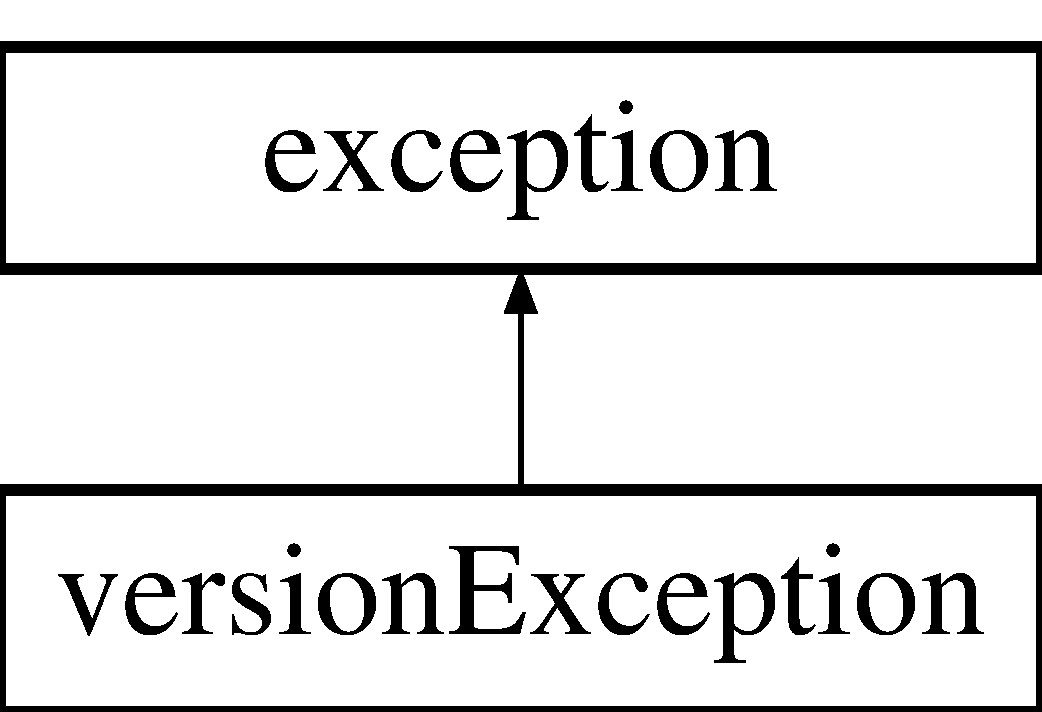
\includegraphics[height=2.000000cm]{classversion_exception}
\end{center}
\end{figure}


The documentation for this class was generated from the following file\-:\begin{DoxyCompactItemize}
\item 
M\-P\-A\-G\-S\-Cipher/Command\-Line\-Helpers.\-cpp\end{DoxyCompactItemize}

\hypertarget{struct_version_exception}{\section{Version\-Exception Struct Reference}
\label{struct_version_exception}\index{Version\-Exception@{Version\-Exception}}
}


The documentation for this struct was generated from the following file\-:\begin{DoxyCompactItemize}
\item 
M\-P\-A\-G\-S\-Cipher/Custom\-Exceptions.\-cpp\end{DoxyCompactItemize}

\hypertarget{class_vigenere_cipher}{\section{Vigenere\-Cipher Class Reference}
\label{class_vigenere_cipher}\index{Vigenere\-Cipher@{Vigenere\-Cipher}}
}


{\ttfamily \#include $<$Vigenere\-Cipher.\-hpp$>$}

\subsection*{Public Member Functions}
\begin{DoxyCompactItemize}
\item 
\hyperlink{class_vigenere_cipher_add794fab3207409dcd5962319559b694}{Vigenere\-Cipher} (std\-::string constructorkey, Cipher\-Mode mode)
\item 
\hypertarget{class_vigenere_cipher_a0277fd4f60a7dd6384f4042de8cad34d}{void \hyperlink{class_vigenere_cipher_a0277fd4f60a7dd6384f4042de8cad34d}{create\-Ciphers} ()}\label{class_vigenere_cipher_a0277fd4f60a7dd6384f4042de8cad34d}

\begin{DoxyCompactList}\small\item\em creates and fills the vector of Caesar\-Ciphers \end{DoxyCompactList}\item 
\hypertarget{class_vigenere_cipher_a32b3cd7e3c27f1f77b2bbabd39d88687}{Cipher\-Mode \hyperlink{class_vigenere_cipher_a32b3cd7e3c27f1f77b2bbabd39d88687}{get\-Mode} ()}\label{class_vigenere_cipher_a32b3cd7e3c27f1f77b2bbabd39d88687}

\begin{DoxyCompactList}\small\item\em returns the Cipher\-Mode of the Vigenere Cipher \end{DoxyCompactList}\item 
\hypertarget{class_vigenere_cipher_a56da7859a8a8d2b2f9b05e59b9ab43f1}{void \hyperlink{class_vigenere_cipher_a56da7859a8a8d2b2f9b05e59b9ab43f1}{make\-It\-Look\-Nice} (std\-::string \&msg)}\label{class_vigenere_cipher_a56da7859a8a8d2b2f9b05e59b9ab43f1}

\begin{DoxyCompactList}\small\item\em A function which isn't implemented but included to match other Cipher classes. \end{DoxyCompactList}\item 
std\-::string \hyperlink{class_vigenere_cipher_a4bc1e285ea48d73bc100f1cf247ce5a4}{encrypt} (std\-::string msg)
\end{DoxyCompactItemize}
\subsection*{Public Attributes}
\begin{DoxyCompactItemize}
\item 
std\-::vector$<$ \hyperlink{class_caesar_cipher}{Caesar\-Cipher} $>$ \hyperlink{class_vigenere_cipher_a689c8803694f5ed4284f38f090540c89}{cipher\-\_\-\-Holder\-\_\-}
\end{DoxyCompactItemize}


\subsection{Detailed Description}
\hyperlink{class_vigenere_cipher}{Vigenere\-Cipher} contains all possible 26 Caesar Ciphers and selects which to use based on the keyword stored in key\-\_\- 

\subsection{Constructor \& Destructor Documentation}
\hypertarget{class_vigenere_cipher_add794fab3207409dcd5962319559b694}{\index{Vigenere\-Cipher@{Vigenere\-Cipher}!Vigenere\-Cipher@{Vigenere\-Cipher}}
\index{Vigenere\-Cipher@{Vigenere\-Cipher}!VigenereCipher@{Vigenere\-Cipher}}
\subsubsection[{Vigenere\-Cipher}]{\setlength{\rightskip}{0pt plus 5cm}Vigenere\-Cipher\-::\-Vigenere\-Cipher (
\begin{DoxyParamCaption}
\item[{std\-::string}]{constructorkey, }
\item[{Cipher\-Mode}]{mode}
\end{DoxyParamCaption}
)}}\label{class_vigenere_cipher_add794fab3207409dcd5962319559b694}
Create a new Vigenere


\begin{DoxyParams}{Parameters}
{\em constructorkey} & the key to the cipher. \\
\hline
{\em mode} & whether to 'Encrypt' or 'Decrypt' \\
\hline
\end{DoxyParams}

\begin{DoxyCode}
14   :mode\_\{decrypt\_mode\}
15    \{
16      std::string transformedKey\{\textcolor{stringliteral}{""}\};
17      \textcolor{keywordtype}{char} in\_char\{\textcolor{charliteral}{'x'}\};
18      \textcolor{keywordflow}{for}(\textcolor{keywordtype}{size\_t} pos=0; pos < thekey.length(); pos++)\{
19        in\_char = thekey.at(pos);
20        transformedKey += transformChar(in\_char);
21      \}
22      key\_ = transformedKey;
23      \hyperlink{class_vigenere_cipher_a0277fd4f60a7dd6384f4042de8cad34d}{createCiphers}();
24        \}
\end{DoxyCode}


\subsection{Member Function Documentation}
\hypertarget{class_vigenere_cipher_a4bc1e285ea48d73bc100f1cf247ce5a4}{\index{Vigenere\-Cipher@{Vigenere\-Cipher}!encrypt@{encrypt}}
\index{encrypt@{encrypt}!VigenereCipher@{Vigenere\-Cipher}}
\subsubsection[{encrypt}]{\setlength{\rightskip}{0pt plus 5cm}std\-::string Vigenere\-Cipher\-::encrypt (
\begin{DoxyParamCaption}
\item[{std\-::string}]{msg}
\end{DoxyParamCaption}
)}}\label{class_vigenere_cipher_a4bc1e285ea48d73bc100f1cf247ce5a4}
\begin{DoxyReturn}{Returns}
the encrypted/decrypted string 
\end{DoxyReturn}

\begin{DoxyParams}{Parameters}
{\em msg} & the message to be used \\
\hline
\end{DoxyParams}

\begin{DoxyCode}
47                                               \{
48 
49   \textcolor{comment}{//generate keyphrase of the right length}
50   
51 
52   std::string keyphrase\{\textcolor{stringliteral}{""}\};
53 
54   \textcolor{keywordflow}{while}(keyphrase.length() < msg.length() )\{
55 
56     keyphrase += key\_;
57   \}
58   \textcolor{keywordtype}{size\_t} need\_to\_erase = keyphrase.length() - msg.length();
59 
60   keyphrase.erase(msg.length(), need\_to\_erase);
61 
62   std::cout << \textcolor{stringliteral}{"keyphrase: "} << keyphrase << std::endl;
63 
64   std::string encrypted\{\textcolor{stringliteral}{""}\};
65 
66 
67 
68   \textcolor{keywordflow}{for}(\textcolor{keywordtype}{size\_t} pos=0; pos < msg.length(); pos++)\{
69 
70     
71     \textcolor{keywordtype}{char} fowl = (keyphrase.c\_str())[pos];
72     \textcolor{keywordtype}{int} ming = int(fowl);
73     ming -= 65;
74     std::string doodah = msg.substr(pos, \textcolor{keywordtype}{size\_t}(1));
75      encrypted += \hyperlink{class_vigenere_cipher_a689c8803694f5ed4284f38f090540c89}{cipher\_Holder\_}[ming].encrypt(doodah);
76 
77    \}
78   \textcolor{keywordflow}{return} encrypted;
79 \}
\end{DoxyCode}


\subsection{Member Data Documentation}
\hypertarget{class_vigenere_cipher_a689c8803694f5ed4284f38f090540c89}{\index{Vigenere\-Cipher@{Vigenere\-Cipher}!cipher\-\_\-\-Holder\-\_\-@{cipher\-\_\-\-Holder\-\_\-}}
\index{cipher\-\_\-\-Holder\-\_\-@{cipher\-\_\-\-Holder\-\_\-}!VigenereCipher@{Vigenere\-Cipher}}
\subsubsection[{cipher\-\_\-\-Holder\-\_\-}]{\setlength{\rightskip}{0pt plus 5cm}std\-::vector$<${\bf Caesar\-Cipher}$>$ Vigenere\-Cipher\-::cipher\-\_\-\-Holder\-\_\-}}\label{class_vigenere_cipher_a689c8803694f5ed4284f38f090540c89}

\begin{DoxyParams}{Parameters}
{\em cipher\-\_\-\-Holder\-\_\-} & a vector of all Caesar Ciphers \\
\hline
\end{DoxyParams}


The documentation for this class was generated from the following files\-:\begin{DoxyCompactItemize}
\item 
M\-P\-A\-G\-S\-Cipher/Vigenere\-Cipher.\-hpp\item 
M\-P\-A\-G\-S\-Cipher/Vigenere\-Cipher.\-cpp\end{DoxyCompactItemize}

%--- End generated contents ---

% Index
\newpage
\phantomsection
\addcontentsline{toc}{chapter}{Index}
\printindex

\end{document}
